\chapter{Experimental Setup}
\label{exp}

\section{CERN}
\label{exp:CERN}
The European Organization for Nuclear Research, or CERN, is an
international laboratory just outside Geneva, Switzerland.  
It was founded in 1954 as a collaborative effort between twelve European 
countries.  
It now has twenty member states, as well as many observer 
and other non-member states, and is one of the world's major 
particle physics facilities.  
%Europe, founded 1959?, maybe little significant history.  

\section{Large Hadron Collider}
\label{exp:LHC}
%All the good stats on the LHC: circumference, (place,) dipole design, magnets, magnetic field.  
%Design energy and luminosity.  how beam is actually accelerated.  
%And pictures!  diagram of LHC, diagram of magnets?  just going through prelim diagrams here!
%maybe done need one of magnets

%Accelerator chain? LINAC2->PS boosters->PS->SPS->LHC
% http://public.web.cern.ch/public/en/Research/AccelComplex-en.html

% iCMS on Nov. 20, 2010
% Maximum luminosity = 204.78 1030 cm-2s-1
% Recorded luminosity = 43.17 pb-1

The Large Hadron Collider (LHC) \cite{LhcMachine}
is a circular particle accelerator near Geneva, Switzerland, 
with a circumference of 27 km. 
Two proton beams circulate in opposite directions around the ring
and cross at several points, which are home to large particle detectors.  
Figure \ref{fig:LHCDiagram} shows a diagram of the LHC layout.  
The two general-purpose detectors, CMS and ATLAS, sit on opposites sides of the ring, 
while the two smaller specialty detectors, LHCb and ALICE, 
sit at the interaction points to either side of ATLAS.  
Each beam consists of a series of proton bunches, 
with a maximum of 2835 ``buckets'' in the beam to be filled by bunches.  
The bunch structure is such that the nominal bunch crossing rate is 40 MHz.  

The proton beams are accelerated from injection energy by a 
radio frequency (RF) chamber, 
which provides an energy boost with each circulation of the beam
until the collision energy is achieved.  
The beams are steered around the ring by 8-Tesla magnetic fields produced in 
15-meter-long superconducting niobium-titanium dipole magnets,
and focused by quadrupole magnets, 5-7 m long.  
The LHC uses a design in which both proton beampipes are contained in the same housing,
allowing the same liquid helium cooling system to serve both.  

The LHC began colliding proton beams in March 2010, 
quickly reaching its 2010 center-of-mass operating energy of 7 TeV
(3.5 TeV per proton beam).  
At this energy it delivered over 47 pb$^{-1}$ of collisions, 
with a maximum instantaneous luminosity of over 2*10$^{32}$ cm$^{-2}$s$^{-1}$.  
The LHC maximum design energy is 14 TeV (7 TeV per beam), 
and its design luminosity is 10$^{34}$ cm$^{-2}$s$^{-1}$.  

 \begin{figure}[htb]
  \begin{center}
    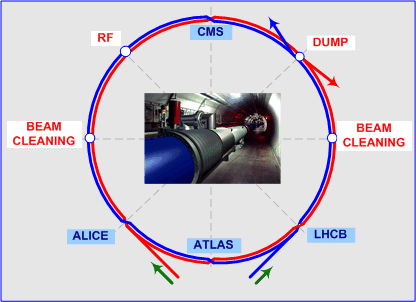
\includegraphics[width=360pt]{Figures/lhc-schematic-ml.png} 
  \end{center}
  \caption[Diagram of the LHC layout]{Diagram of the LHC layout.}
  \label{fig:LHCDiagram}
 \end{figure}


\section{Compact Muon Solenoid}
\label{exp:CMS}
%SUBDETECTORS: material, coverage, resolution (spatial and energy/mom/whatever)

%Important stats on CMS: height, weight, etc.  diagram of detector.  
%Current status on detector, data-taking, event display -- here? or after everything explained?  
%At collision energy (7 TeV), CMS recorded 35 pb-1 of good data (but 43 recorded sez lumi plot)

The Compact Muon Solenoid (CMS) \cite{CmsExperimentAtCernLHC}
is one of the two general-purpose experiments for the LHC.  
Figures \ref{fig:CMSDiagram3D} and \ref{fig:CMSDiagramFlat} 
show the structure of the CMS detector.  
It is cylindrical, 21.5 m long and with a 15-m diameter, and weighs 12,500 tons.  
The overall structure of the detector is formed by the iron yoke framework surrounding the inner detector,
with the central section, the ``barrel'', divided into five ring-shaped slices, 
while each end of the cylinder, or ``endcap'', consists of several circular plates.  
These sections fit around the solenoid and inner detector, enclosing it completely.  

Particle detection is done by several dedicated subdetectors.  
The electromagnetic and hadronic calorimeters fit inside the solenoid, 
with the tracking system inside the calorimeters.  
The three components of the muon system are outside the solenoid,
integrated with the iron magnetic field return yoke:
the drift tube chambers, resistive plate chambers,
and cathode strip chambers.  

%Figure: CMS diagram, Fig. \ref{fig:CMSDiagram}
% also nice one in HLT paper

 \begin{figure}[htb]
  \begin{center}
    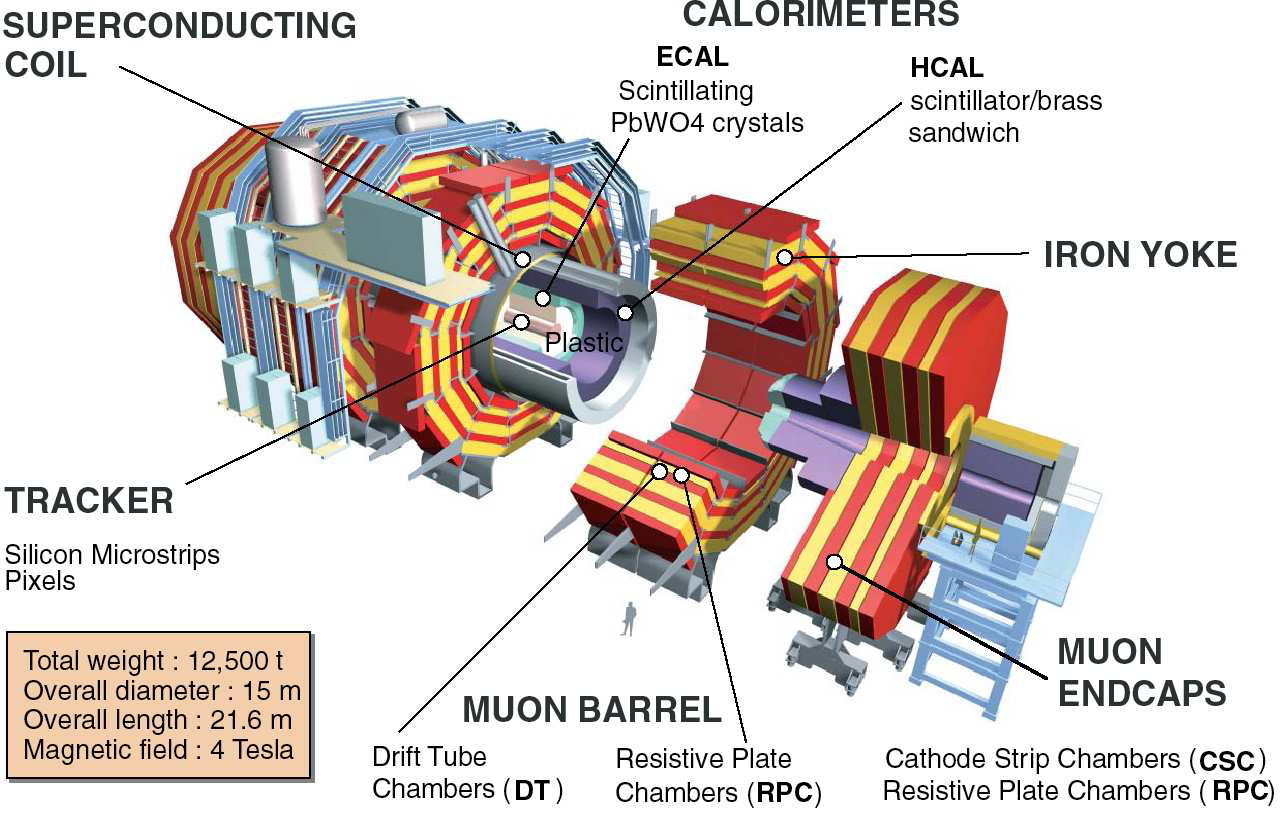
\includegraphics[width=360pt]{Figures/CMSncLabels.png}
  \end{center}
  \caption[Expanded view of the CMS detector]{Expanded view of the CMS detector, showing the ring and slice structure as well as the placement of each subsystem.}
  \label{fig:CMSDiagram3D}
 \end{figure}

 \begin{figure}[htb]
  \begin{center}
    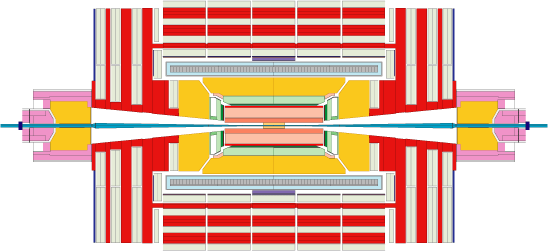
\includegraphics[width=360pt]{Figures/Longnc.png}
  \end{center}
  \caption[Cross-sectional view of the CMS detector]{Cross-sectional view of the CMS detector.}
  \label{fig:CMSDiagramFlat}
 \end{figure}

\subsection{Detection of Particle Interactions}
\label{exp:particleDetection}
%Figure: Particle detection in CMS, Fig. \ref{fig:CMSParticles}

 \begin{figure}[htb]
  \begin{center}
    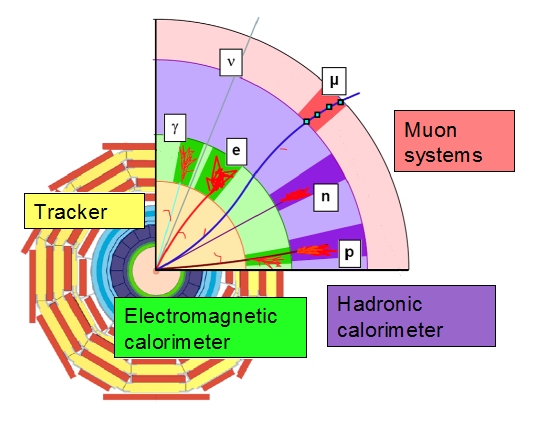
\includegraphics[width=360pt]{Figures/CMSParticles.png}
  \end{center}
  \caption[Detection of particles in the CMS detector]{Detection of particles in the CMS detector.}
  \label{fig:CMSParticles}
 \end{figure}

The various parts of the CMS detector work together to differentiate
the end-products of proton interactions.  
As the end-product particles traverse their outward trajectory,
they pass through the different subdetectors in turn.
Figure \ref{fig:CMSParticles} shows how end-product particles 
interact with the subsystems of the CMS detector.  
The innermost subdetector is the tracker, 
which reconstructs a particle's track through it
from a set of points where it detected an interaction.  
The tracker only registers particles with an electric charge;%, 
%such as electrons or muons;
neutral particles pass through undetected.  
The electromagnetic calorimeter detects particles that interact
primarily electromagnetically.%, 
%such as electrons and photons.
%Since pions, which are hadrons, can interact in the ECAL like eg particles, 
%have ES in endcap BUT PUT THIS IN ECAL SECTION
In this way the first two ``layers'' of the detector can differentiate
electrons from photons: 
both are seen in the electromagnetic calorimeter, 
but only electrons leave traces in the tracker.
Outside of the electromagnetic calorimeter is the hadronic calorimeter,
which primarily detects hadrons.  
Hadrons are also detected in the electromagnetic calorimeter,
but they leave the largest signature in the hadronic calorimeter,
which differentiates the hadrons from the electromagnetic particles
like electrons and photons.  
Hadrons are often found in large quantities called ``jets'' 
(see Section~\ref{theory:HigherOrderDiagrams}),
so summing together the energy deposits from sizable electromagnetic 
and hadronic calorimeter regions is important in event reconstruction.  
Surrounding the tracker and the calorimeters is the solenoid,
which generates the magnetic field.
The charge of a particle can be determined from which way it
bends in the magnetic field.
Finally, outside the solenoid and interwoven with the panels of the 
iron return yoke, is the muon system.  
Muons leave traces in the inner subdetectors, 
but they are the only particles to live long enough to reach the
muon system.
This differentiates them from the other particles detected by 
the inner subdetectors.  
Since the muon system is outside the solenoid, 
the magnetic field points in the opposite direction,
and hence the muon trajectories bend in the other direction
from what they had inside the solenoid.  
The last category of end-product, neutrinos, 
generally cannot be detected.
However, their direction and energy in the radial plane 
can be reconstructed 
by summing the energy of all the particles in the event.
Because the initial protons have zero momentum in the radial plane, 
and momentum is always conserved, 
any significant ``missing'' component to the final energy
can be taken to be due to a neutrino.  

A CMS event display from 2010 running can be seen in Fig. \ref{fig:EventDisplay}.  

 \begin{figure}[htb]
  \begin{center}
    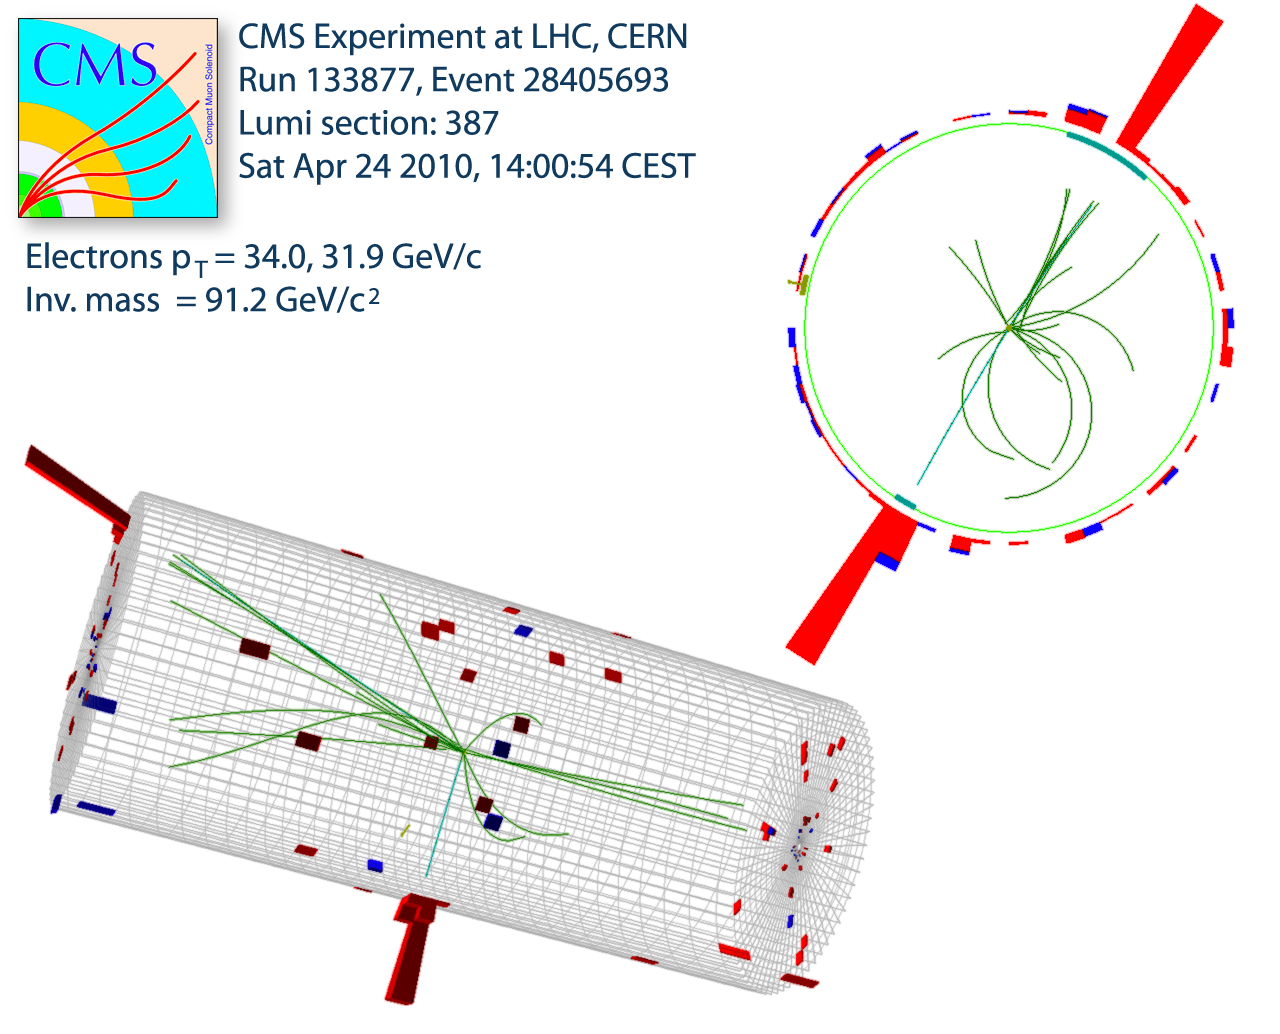
\includegraphics[width=360pt]{Figures/zee-133877-28405693-full.png}
  \end{center}
  \caption[Three-dimensional display of a \Zee event in the CMS detector]{Three-dimensional display of a \Zee event in the CMS detector.}
  \label{fig:EventDisplay}
 \end{figure}

\subsection{Coordinate System} %define eta and phi earlier? YES
\label{exp:coords}
A standardized set of coordinates is used to describe points and directions within the CMS detector.  
The origin of the coordinate system is at the interaction point,
with the $x$-direction pointing horizontally south towards the LHC center
(ignoring the slight tilt of the LHC ring with respect to the vertical),
and the $y$-direction pointing directly upwards.  
The $z$-axis points horizontally west along the beam direction,
and the magnetic field inside the solenoid points in the positive $z$-direction.  
The azimuthal angle $\phi$, measured in the $x$-$y$ plane and ranging from $-\pi$ to $+\pi$ radians, 
is oriented such that $ \phi = 0 $ is equivalent to the positive $x$-axis
and $ \phi = \pi/2 $ is equivalent to the positive $y$-axis.  
The longitudinal angle $\theta$ is measured from the positive $z$-axis, 
and the sign of $ \eta = -\ln\tan(\theta/2)$ is equal to the sign of $z$.  

\subsection{Magnet}
\label{exp:magnet}
%Stats about the magnet!  how much field, how much current, weight, what it's made of,
%what makes it special

Since charged particles bend in a magnetic field, 
particle detectors use some sort of magnetic field to determine 
the charges of decay products.  
CMS uses a solenoid, or electromagnet in the shape of a coil, 
to produce a uniform magnetic field in the detector's inner region.  
The magnet coil is 12.5 m long with a 6 m diameter, 
and it weighs 220 metric tons.  
The CMS solenoid is made of a superconducting material, 
a niobium-titanium alloy, 
to handle the large amount of current necessary: 
it generates a field of 4 Tesla using 
a current of almost 20 kA in a four-layer winding.

The magnetic field is returned through a 10,000 metric ton iron yoke, 
which also serves as a support structure for the detector.  
The yoke consists of three concentric cylinders divided into the same 
5-ring barrel and 3-disk endcap structure as mentioned previously.  

\subsection{Tracker}
\label{exp:tracker}
The purpose of the tracker is to detect the 
tracks from end-product particles;
only those which are charged can be detected in the tracker.  
The CMS tracker contains 75 million channels
and is specifically designed to get good performance 
using only a small number of hits per track.
%very fine accuracy (10 um) in order to reconstruct vertices and decays (?)
It is the innermost layer of the CMS detector
and is made up of two different systems: 
the pixel detector, 
which is closest to the interaction point and hence has the finer granularity, 
and the strip tracker, 
covering the volume out to the calorimeter. 
Both systems are made of silicon and register charged particles in the same way. 
When a charged particle passes through the silicon,
it knocks electrons out of the material, 
creating a net positive charge.  
The electric current needed to return the silicon
to its neutral state is measured and amplified
by the readout electronics.  
This readout technology is fast compared to the 
25 ns bunch spacing of the LHC.  
A single track is reconstructed by stringing together
the measurements from each of the layers.  

\subsubsection{Pixels}
\label{exp:pixels}
The silicon pixel detector has a very fine accuracy
due to the high density of tracks near the interaction point.  
It consists of 65 million readout channels 
arranged on modules in several layers around the interaction point.
In the barrel, the layers are cylindrical and situated at
radii of 4, 7, and 11 cm, 
while each endcap has two disks, at 6 and 15 cm from the
interaction point. 
Each module consists of a rectangular array of 100 $\mu$m x 150 $\mu$m pixels, 
with a resolution of ~15 $\mu$m.  
The pixels on each module are read out by a dedicated chip attached 
to the module. 
The chip contains readout unit cells, one corresponding to each pixel,
which are connected to the pixels with a small bump of solder 
in the so-called bump-bonding method.  

 \begin{figure}[htb]
  \begin{center}
    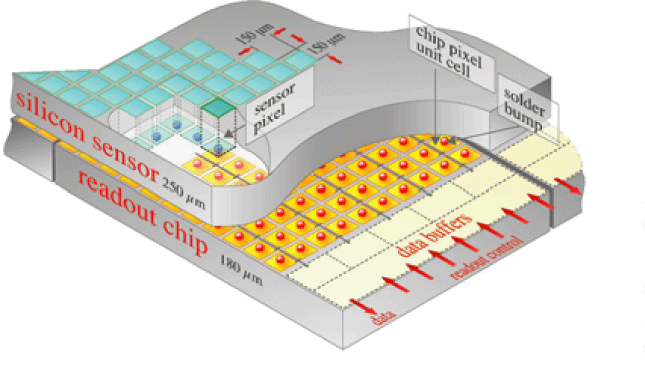
\includegraphics[width=360pt]{Figures/tracker-Pixelement.png}
  \end{center}
  \caption[Structure of pixel detector layers]{Structure of pixel detector layers.}
  \label{fig:PixelLayers}
 \end{figure}

\subsubsection{Strips}
\label{exp:strips}
The silicon strip detector consists of 10 million channels
arranged in 10 layers of strips, 
in both the barrel and the endcap,
and extends to a radius of 130 cm from the interaction point
and to an $|\eta|$ value of 2.5.  
The track density at this stage is much less than in the pixel detector,
so the granularity does not need to be as fine.
%don't need to have quite as minute accuracy here, since particles are already on their way out.
%detection principle same as for pixels.
Each strip is between about 12 and 16 cm long,
with a resolution ranging from ~15 $\mu$m in the inner barrel
to ~50 $\mu$m in the outer tracker.  
The strips are arranged in modules of 6 inches in length, 
with the geometry of each module dependent 
on its position in the tracker.  
The strip tracker consists of four different parts: 
the tracker inner barrel (TIB) with four layers of strips reaching to a radius of 50 cm, 
the tracker inner endcap disks (TID) with three layers to +-90 cm in $z$, 
the tracker outer barrel (TOB) with six layers to 1.16 m radially, 
and the tracker outer endcap (TEC) with nine layers, extending to +-2.8 m in $z$. 
Several of the layers are double-sided: 
they contain two sets of silicon modules.  
The two sets of modules are arranged in a stereo
geometry to accurately measure the longitudinal
(or radial, in the endcap) coordinate of the hit 
as well as the azimuthal.  
%explain each, including double-layered stuff.

%cooled to -20 C (also pixels?) to prevent radiation damage (damage doesn't propagate, look up details)

 \begin{figure}[htb]
  \begin{center}
%    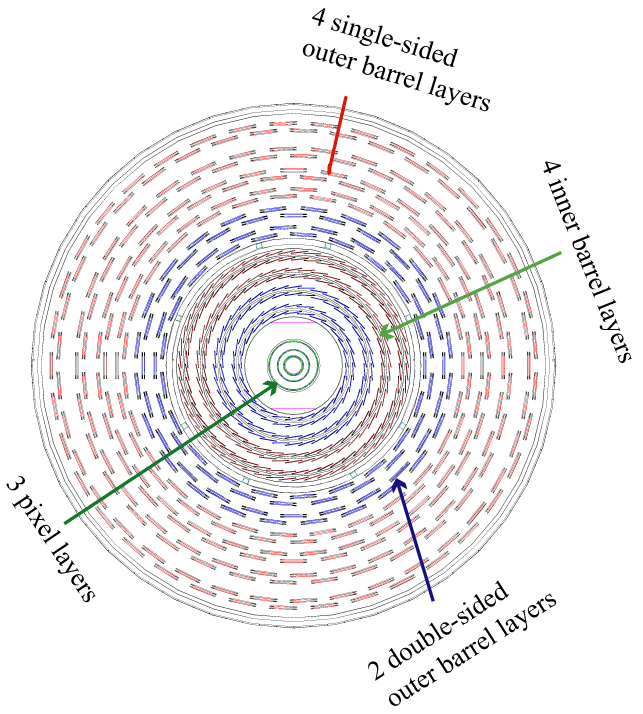
\includegraphics[width=360pt]{Figures/tracker-Barrel.png}
    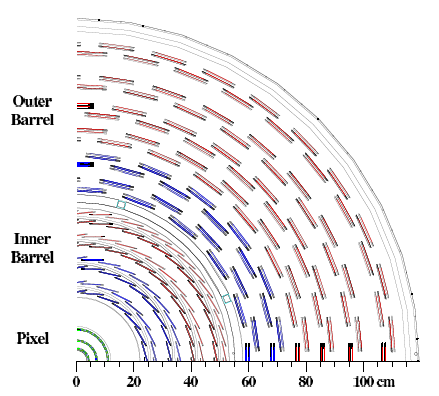
\includegraphics[width=360pt]{Figures/tracker-schematic.png}
  \end{center}
  \caption[Diagram of layers in tracker barrel]{Diagram of layers in tracker barrel.}
  \label{fig:TrackerBarrel}
 \end{figure}

\subsection{Calorimeters}
\label{exp:cal}
The general purpose of a calorimeter 
is to measure energy passing through it.  
CMS measures the energy of decay products 
with a scintillating electromagnetic calorimeter (ECAL),
situated just outside the tracker,
and a sampling hadronic calorimeter (HCAL),
surrounding the ECAL.  
Both calorimeters are contained within the solenoid.  
This solves a problem seen in other detector designs, 
in which energy lost in the magnet material leads 
to an uncertainty in the energy measurement.  

\subsubsection{ECAL}
\label{exp:ECAL}
The ECAL is made up of ~76,000 lead tungstate crystals,
arranged in a cylindrical barrel and disk-shaped endcap geometry.  
The barrel is divided into 18 sections in $\phi$ and 
two in $\eta$, called supermodules.  
Each endcap is divided into two half-disks, called dees.  
Each lead tungstate crystal is 
2.2 cm x 2.2 cm wide and 23 cm long for the barrel, 
and 3 cm x 3 cm wide and 22 cm long in the endcap.  
The dimensions were chosen such that the width 
of each crystal is approximately the characteristic size of 
an electromagnetic shower within it 
(Moliere radius of 2.19 cm),
and the length is ~25 times the radiation length 
of the material (0.89 cm for lead tungstate).  
The crystals are oriented with the long axis
directed towards the interaction point.  
However, to avoid particles being lost in the cracks 
between the crystals,
the crystals are offset by 3 degrees in both the 
$\phi$ and $\eta$ directions.  
An electromagnetically-interacting particle will 
induce a shower inside the crystals, 
and the resulting light is captured by 
photodetectors situated at the back of each crystal.  
The energy resolution was measured to be 
\[
%INSERT LONG FUN EQUATION FROM P.120(147) OF DETECTOR PAPER HERE
\left(\frac{\sigma}{E}\right)^2 = \left(\frac{2.8\%}{\sqrt{E}}\right)^2 + \left(\frac{0.12}{E}\right)^2 + \left(0.30\%\right)^2
\]

A preshower detector, consisting of lead radiators 
and silicon sensors, 
is situated on the face of each endcap.  
The preshower serves to identify electron pairs due to low-energy 
pion decays and differentiate them from more 
interesting signatures.  
Pions typically decay on the scale 
of the distance between the interaction point and the 
ECAL endcap;
therefore there is no preshower detector for the barrel, 
which is too close to the interaction point.  

\subsubsection{HCAL}
\label{exp:HCAL}
%HCAL resolution of energy: CMS NOTE 2006/036, but it's only
%MC and also not just one equation.  can give value
%quoted in abstract.  also, incl ecal: it's for reco jets
%OR can take value from prelim, but don't remember where it came
%from: look in HCAL TDR
%ORRRR: not important because not in detector paper, and
%couldn't find it in tdr? (which is confusing in any case)
The hadronic calorimeter surrounds the ECAL and 
covers $|\eta| < 3$ in the barrel and endcap (HB/HE) 
and up to $|\eta| < 5$ in the forward calorimeter (HF),
both within the magnet coil.
Additionally, the outer calorimeter (HO) is situated 
outside the solenoid and serves to detect 
and measure any leak-through.
In general HCAL uses sampling calorimeter technology, 
with brass and scintillator layers interleaved 
in the barrel and endcap, 
and steel plates and quartz fibers for HF; 
quartz was used in the forward region 
because of its ability to 
withstand very high particle fluxes.  
In a sampling calorimeter, the layers of metal absorber 
induce particle showers, which are then 
``sampled'' by the layers of scintillator 
attached to photodetectors.  
Not all of the energy is directly detected, 
some being lost in the metal,
so the energy measurement is scaled using 
experimentally-determined factors.  
The depth of the HCAL 
in terms of interaction length 
varies between 5.82 $\lambda_I$ at $\eta = 0$ and 
10.6 $\lambda_I$ at the edge of HB and throughout 
the endcap, 
with the ECAL adding 1.1 $\lambda_I$.  
The HO extends the HCAL depth to at least 
11.8 $\lambda_I$ in the barrel, 
with the magnet material acting as the absorber for 
the HO scintillator layer.  
(An additional layer of iron and 
a second scintillator exist
at the $\eta = 0$ ring, 
where the HB depth is the least.)
Since there is no ECAL in the forward region, 
the HF is equipped to distinguish electromagnetic 
objects from hadronic jets with different 
lengths of quartz fibers.  
The long fibers reach the entire depth of HF, 
while the short fibers only start halfway through 
the detector.
Since electromagnetic showers tend to occur in the 
first half of the detector, 
and hadronic showers throughout the full HF, 
a shower detected only by the long fibers 
is likely to be electromagnetic in nature.  

\subsection{Muon System}
\label{exp:muons}
The CMS muon system serves to identify muons, 
which are the only particles that leave a signature 
very far from the interaction point,
and also to measure their momentum.  
The system is situated outside the magnet coil, 
within the iron return yoke, 
and provides coverage up to $|\eta| < 2.4$.  
The return yoke also functions as an absorber 
to filter out backgrounds to the muon signal.  
The muon system consists of three separate subsystems: 
drift tube chambers (DTs) in the barrel up to $|\eta| < 1.2$, 
cathode strip chambers (CSCs) in the endcap 
with an $\eta$ range $ 0.9 < |\eta| < 2,4$, 
and resistive plate chambers (RPCs) %providing redundancy 
in the region $ |\eta| < 1.6$.  

The DTs are used in the barrel due to 
relatively low muon rates in this area, 
in addition to a uniform magnetic field in the 
return yoke.  
Four stations of chambers are interspersed 
with the iron frame to form
concentric cylinders around the beam pipe, 
with a total of ~172,000 detection wires.  
Orthogonal positioning of the wires 
within each chamber provides measurement of 
both azimuthal and longitudinal position.  
Each wire detects charge that drifts toward it 
due to an applied voltage when a muon ionizes 
the surrounding gas, as illustrated in 
Figure \ref{fig:DTconcept}.  
Neighboring chambers overlap 
to ensure full coverage.  

 \begin{figure}[htb]
  \begin{center}
    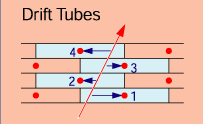
\includegraphics[]{Figures/muon-DT-concept.png}
  \end{center}
  \caption[Conceptual diagram of drift tube chambers]{Conceptual diagram of drift tube chambers.}
  \label{fig:DTconcept}
 \end{figure}

The CSCs are used in the endcap, 
where the muon rate and overall particle flux 
are higher.  
Cathode strips in each chamber 
measure the $\phi$-position of a hit, 
while anode wires oriented perpedicularly measure 
the $\eta$-position.  
There are on the order of 200,000 readout channels 
for each type of measurement.  
Four stations of CSCs are used in each endcap; 
each muon in the range $1.2 < |\eta| <2.4$ crosses either 
3 or 4 stations.  
For $|\eta|$ between 0.9 and 1.2, muons are detected 
both by the CSCs in the endcap and the DTs in the barrel.  
Coverage is provided by overlapping layers of chambers 
at each station.  

 \begin{figure}[htb]
  \begin{center}
    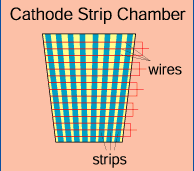
\includegraphics[]{Figures/muon-CSC-structure.png}
  \end{center}
  \caption[Diagram of cathode strip chamber]{Diagram of cathode strip chamber, showing the cathode strips and anode wires for measuring the $\phi$ and $\eta$ coordinates, respectively.}
  \label{fig:CSCstructure}
 \end{figure}

The RPCs provide redundancy for the previous 
two systems as well as a faster response time 
in place of a highly accurate position measurement.  
The RPCs measure the timing of a hit with a 
1 ns resolution, compared to the 25 ns LHC bunch spacing 
and hundreds of ns drift time in the drift chambers.  
Six layers of RPCs are interspersed with the 
drift tubes in the barrel, 
while three layers are used in the endcap 
with the CSCs.  
Again, overlapping chambers ensures full coverage.  
Each chamber consists of two or three double-gap 
modules, each of which has a single readout module 
between two thin gas chambers.  
The readout module consists of metal strips, 
which capture the electric charge created when 
a muon ionizes the gas, causing an avalanche of charge.  
Figure \ref{fig:RPClayers} shows a diagram of the structure.  

 \begin{figure}[htb]
  \begin{center}
    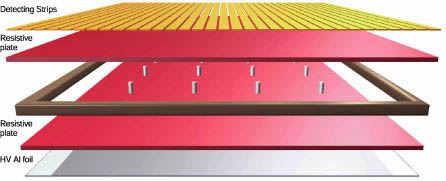
\includegraphics[width=360pt]{Figures/muon-RPClayers.jpg}
  \end{center}
  \caption[Diagram of resistive plate chamber]{Diagram of resistive plate chamber.}
  \label{fig:RPClayers}
 \end{figure}

Overall, the muon system has a momentum resolution 
of 9\% for relatively moderate-$p_T$, low-$\eta$ muons, 
and ranging from 15\% to 40\% for very-high-$p_T$ muons.  
When combined with the information from the inner tracker, 
however, this resolution improves to ~1\% and 5\%, respectively.  

\subsection{Trigger}
\label{exp:trigger}
The purpose of the CMS trigger is to 
identify potentially interesting events.  
Storing the data from every collision is unfeasible; 
resources allow only a very small fraction of events to be kept.  
Therefore the trigger reduces the effective event rate, 
keeping only the events with an interesting signature, 
for example a large energy deposit.  
There are two levels to the CMS trigger.  
The Level-1 Trigger uses hardware-implemented algorithms to 
reduce the event rate from the LHC collision frequency of 40 MHz 
to a maximum of 100 kHz; 
this must be done quickly since the initial event rate is high. 
The High-Level Trigger reduces the rate further to ~200 Hz, %(OR 100??)
using a computer farm to process each event in more detail; 
having a lower input rate, it can afford more processing time per event.  

%Picture: Overall diagram of trigger

\subsubsection{Level-1 Trigger}
\label{exp:L1}
%General L1 information, specific electron algorithms in online selection section.  
%time-of-flight stuff!

The Level-1 trigger (L1) \cite{TriggerTDR} 
uses mostly programmable, hardware-based algorithms 
to identify and roughly reconstruct possibly interesting physics objects, 
such as electrons and muons.  
This is done within 3 $\mu$s.  
The structure of the L1 is shown in Figure \ref{fig:L1Structure}.  
Parallel chains process the muon system and calorimeter objects separately. 
Tracking information is not included in the L1, 
which means the L1 algorithms do not distinguish 
between electrons and photons. 
%Subsections on that?  Need to talk about the muon parts, as well as the multi-level calo part.  
The first step of the Level-1 trigger is the generation 
of coarse versions of the readout information 
from each of the muon and calorimeter channels; 
this information is called trigger primitives.  
The trigger primitives are passed to regional trigger systems, 
which combine them into trigger objects.  
The objects for each region are then passed to a global system, 
which picks out the highest-energy (and therefore most interesting) 
objects of each type.
The final set of objects gets passed on to the last level, 
the global trigger, which combines information from both 
the calorimeter and muon chains 
and makes a single decision based on the set of criteria implemented.  
%(Ooh boy, go back to RT2010 stuff!)  

The trigger system must combine all the pieces of information 
according to which bunch crossing they originate from.   
This is complicated by the fact that the time it takes particles 
to reach the outer edge of the muon system 
is about that of the bunch crossing interval.  
In addition, the cable lengths between the subdetectors 
and the trigger subsystems and within the trigger are 
all different, 
and each of the trigger systems has a different processing time.  
Despite these challenges, the timing of each piece of 
the L1 trigger has successfully been tuned to keep everything running 
synchronously.  

%(from ecal section) PICTURES OF SUPERMODULE GEOMETRY -- maybe just for trigger section?

%nice picture of L1 architecture from detector paper

 \begin{figure}[htb]
  \begin{center}
    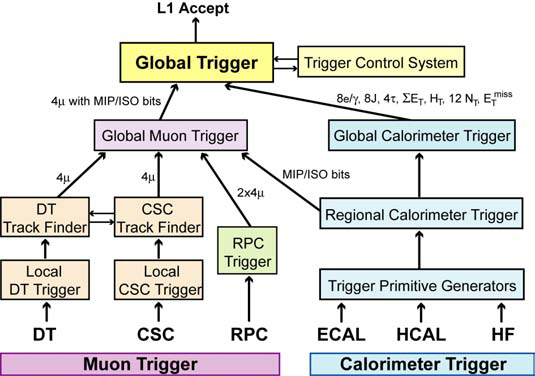
\includegraphics[width=360pt]{Figures/L1structure.png}
  \end{center}
  \caption[Structure of the Level-1 trigger]{Structure of the Level-1 trigger.}
  \label{fig:L1Structure}
 \end{figure}

\subsubsection{Regional Calorimeter Trigger}
\label{exp:RCT}
The Regional Calorimeter Trigger (RCT) \cite{rctTriggerSystem}
was designed and built and is maintained 
by the University of Wisconsin at Madison.  
It sits in eighteen crates in nine racks in the CMS underground electronics room.  
Each crate deals with one slice of $\eta$-$\phi$ space.  
The general purpose of the RCT is to take 
energy information from ECAL and HCAL and combine it 
to generate electron/photon candidates as well as energy sums for 
jet-finding.  
A diagram illustrating the structure of the RCT processing 
is shown in Fig.~\ref{fig:RCTStructure}.  

 \begin{figure}[htb]
  \begin{center}
    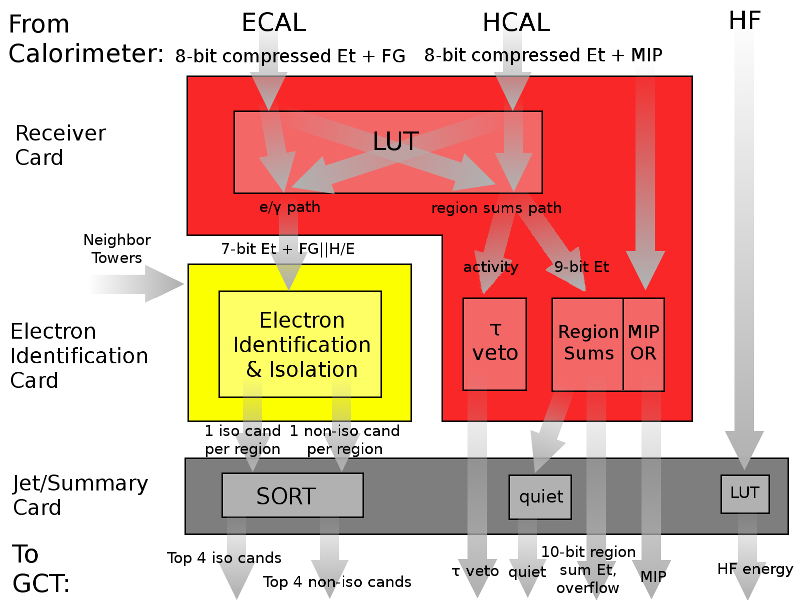
\includegraphics[width=400pt]{Figures/RCT-structure-new-small.png} 
  \end{center}
  \caption[Diagram of the RCT structure]{Diagram of the RCT structure.
  The RCT (Regional Calorimeter Trigger) takes energy 
  information at the tower level from the electromagnetic 
  and hadronic calorimeters.  
  It processes this information to produce 
  regional energy sums, electron candidates, 
  and other regional information to be 
  used in the GCT (Global Calorimeter Trigger) 
  processing further downstream.
  }
  \label{fig:RCTStructure}
 \end{figure}

The information from the calorimeters arrives at the level of trigger towers, 
a larger granularity than that sent to the full readout.  
Each ECAL tower corresponds to an HCAL tower behind it.  
For each ECAL+HCAL tower, the RCT uses lookuptables to 
calculate the total energy sum 
as well as the ratio of HCAL energy to ECAL energy.  
If that ratio is higher than a certain value, 
too much energy has been deposited in the HCAL tower for it to 
contain a probable electron or photon.  
The electron/photon candidates are constructed starting from 
towers whose energy deposit is higher than any of their 
four immediate neighbors.  
This primary tower must not have the ECAL fine grain bit set; 
this fine grain bit indicates a structure in the energy deposit 
inconsistent with an electron or photon.  
The tower's energy is then combined with that of its highest-energy 
neighbor, to account for particles that deposite energy 
in more than one tower; 
this is the energy of the candidate.  
The candidate is then determined to be either ``isolated'' or 
``non-isolated'' depending on the character of the deposits 
in the neighboring towers.  
If the eight towers forming a square around the primary tower 
have two full sides (five contiguous towers) with 
deposits below a configurable threshold (the ``quiet'' threshold), 
and these towers' fine grain bits are not set, 
then the candidate is isolated.  
Otherwise, it is non-isolated.  
The algorithm is illustrated in Figure~\ref{fig:RctEgAlgo}.  
Each crate sorts the isolated and non-isolated candidates found 
according to energy, 
and the four highest-energy of each type are kept and passed on.  

 \begin{figure}[htb]
  \begin{center}
    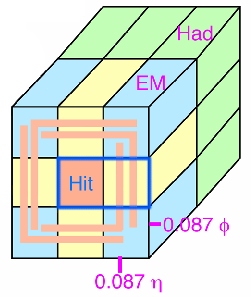
\includegraphics[width=240pt]{Figures/RCT-EG-algo.png} 
  \end{center}
  \caption[Diagram of the RCT electron/photon algorithm]{
    Diagram of the RCT electron/photon algorithm. 
    The candidate is defined as a tower whose four 
    immediate neighbor towers have lower energies.  
    The candidate tower's energy is combined with 
    the energy of its highest-energy neighbor.  
    The candidate is defined as ``isolated'' if 
    five contiguous towers out of the eight 
    surrounding it (two full sides of the square) 
    have energies below a ``quiet'' threshold 
    and do not have the fine grain bit set.  
    Otherwise the candidate is ``non-isolated.''  
  }
  \label{fig:RctEgAlgo}
 \end{figure}

The RCT also calculates the total energy sums 
of square regions of the calorimeter, 
4 trigger towers to a side.  
The topology of the energy deposits in each region 
is examined to determined whether or not the 
deposit is consistent with that from 
a $\tau$ particle that has decayed hadronically, 
i.e. decayed into a jet of hadrons.  
Only deposits above a configurable threshold 
are considered.  
If the deposits in the region make up a 
single, small, contiguous area as shown in 
Figure~\ref{fig:RctTauAlgo},
then they are consistent with a tau.  
In this case the $\tau$ veto bit associated 
with the region is set to false; 
in all other cases, it is set to true.  
In addition, the HCAL sends a bit for each 
HCAL tower indicating whether the deposit 
is consistent with a minimum ionizing particle 
(MIP) or muon.  
If any individual tower's MIP bit is true, 
then the overall MIP bit associated with the region 
is also set to true.  
Otherwise it is set to false.  

 \begin{figure}[htb]
  \begin{center}
    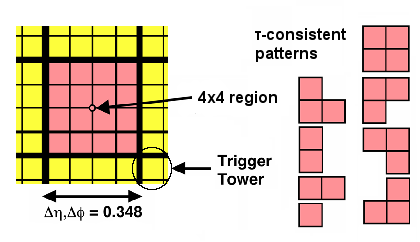
\includegraphics[width=400pt]{Figures/RCT-tau-algo.png} 
  \end{center}
  \caption[Diagram of the RCT $\tau$ algorithm]{
    Diagram of the RCT $\tau$ algorithm. 
    The energy deposits in each region are 
    examined to determine whether they are 
    consistent with that from a $\tau$ 
    that has decayed hadronically.  
    A single small, contiguous region 
    is consistent with a $\tau$. 
  }
  \label{fig:RctTauAlgo}
 \end{figure}

Finally, the RCT sends the regional energy sums 
and the list of possible 
electrons or photons, 
along with the associated bits (MIP, $\tau$), 
to the 
Global Calorimeter Trigger (GCT) level.  
The GCT groups the regional energy sums into jets 
and collects the four highest-energy isolated and 
non-isolated electron/photon candidates, 
and sends this information to the Global Trigger (GT), 
the last step in the chain.  
The Global Trigger makes the final decision on 
whether to accept or reject an event at the Level-1.  
% NEED THE GCT/GT stuff?  talked about it earlier a little


\subsubsection{High-Level Trigger}
\label{exp:HLT}
%General HLT information, specific electron algorithms in online selection section.  

The High-Level Trigger (HLT) \cite{hlt-0512077} 
is implemented on a computer farm in the 
CMS above-ground control room building.  
It serves to reduce the L1 output event rate from ~100 kHz to a rate suitable 
for transfer and storage to disk, around 200 Hz.  
An event must pass the HLT to be analyzed offline.  
The input rate at this stage is lower than that at the Level-1, 
so more time can be afforded to spend on the decision, 
and more detailed reconstruction can be done.  
The HLT uses versions of the standard offline physics-object reconstruction algorithms 
optimized for fast performance.  
The algorithms need to be more accurate than those of the L1, 
but absolute accuracy at the offline reconstruction level is not necessary.  
Still, the HLT algorithms are kept as close to the offline ones as possible.  
Specific algorithms are dealt with in more detail in 
%a later chapter.  
Section~\ref{evSel:HLT}.  

\subsubsection{Trigger Menus}
\label{exp:trigMenus}
Both the L1 and High-Level Triggers use the concept of a trigger menu.  
There are different sets of criteria defining an ``interesting'' event 
at any one time;  
each set of criteria is called a trigger path.  
When an event fulfills all the criteria for a given path, 
that path ``fires'' and the event is accepted.  
Some paths may fire at a higher rate than desired, 
so a prescaling factor is implemented: 
only a fraction of events firing that path is kept.  
For example, a path with a prescale of 5 only 
has 1/5 of its passing events actually saved.  
In this way, events passing a certain path can still 
be studied without taking too much of the available resources.  
The set of paths that are being checked at any given time,
along with their prescale factors,  
is called the trigger menu.  
The Level-1 and High-Level Triggers each have their own 
trigger menus.  
Since the L1 must do things quickly, 
its criteria are simple, 
whereas the HLT may have more complex criteria.  
Passing a given L1 path causes 
related HLT paths to be run on that event.  

%algorithms evolve with luminosity
At the beginning of collision running, 
the event rate was low enough to allow very loose trigger 
menus to be used.  
At the HLT, a ``keep-everything'' pass-through menu 
recorded essentially all activity.  
As the luminosity increased, however, more stringent criteria had 
to be applied to maintain an acceptable event rate, 
for example, raising the amount of energy needed to accept an 
``interesting'' object.  
The successive algorithms have been studied in detail and 
commissioned successfully throughout the 2010 running conditions.  

\subsection{Luminosity}
\label{exp:lumi}
%How the luminosity is measured (definition? or that done earlier in general particle physics section? recap here?)
%What's actually used: HF?? that's in the detector paper, but not much else.  go to twiki, I guess (and that HN thread)

CMS measures luminosity with the forward calorimeter, which sits 
between $|\eta|$ of 3 and 5, close to the beam pipe.  
Two different methods of measurement are used.  
The first method counts the number of occupied towers in the HF 
(above some energy threshold to avoid noise), 
using the principle that that number is proportional to the luminosity.  
However, at high luminosity the number of occupied towers may begin to 
saturate, making this method less accurate.  
The second method does not saturate in this way: 
it measures the total energy deposited in the HF, 
which is also proportional to the luminosity.  
The information from both of these methods is combined into one 
luminosity value.  

Fig. \ref{fig:LuminosityVsTime} shows the total integrated luminosity at CMS 
as a function of time for the 2010 running period \cite{LumiPublicResults2010}.  
The amount of data validated for physics analysis was 
%36.1 $pb^{-1}$.  
36.1 \pb.  

 \begin{figure}[htb]
  \begin{center}
    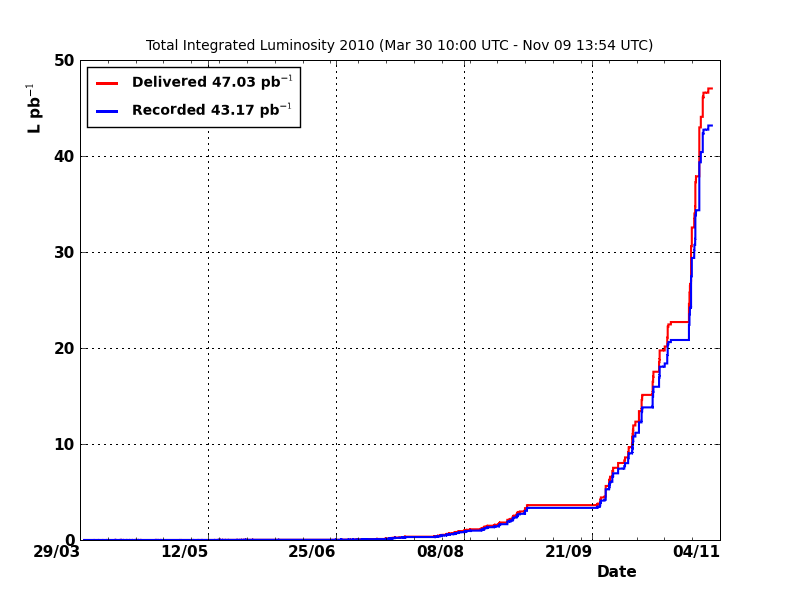
\includegraphics[width=360pt]{Figures/totallumivstime2010.png}
  \end{center}
  \caption[Luminosity collected by CMS as a function of time, 2010]{Luminosity collected by CMS as a function of time, 2010.}
  \label{fig:LuminosityVsTime}
 \end{figure}

% need the DAQ someplace??  online event selection?  or don't really need it?
% really don't need too much in the way of specifics, methinks

